\documentclass[fleqn,11pt]{article}

\usepackage[letterpaper,margin=0.75in]{geometry}

\usepackage{amsmath}
\usepackage{booktabs}
\usepackage{graphicx}
\usepackage{listings}
\usepackage{fancyhdr}
\usepackage{standalone}
\usepackage{pgfplots}
\usepackage{float}
\usepackage{csvsimple}

% \include{data/reaction-time.csv}
 
\pgfplotsset{compat = newest}

\setlength{\parindent}{1.4em}

\pagestyle{fancy}


\begin{document}

\lstset{
  language=Python,
  basicstyle=\small,          % print whole listing small
  keywordstyle=\bfseries,
  identifierstyle=,           % nothing happens
  commentstyle=,              % white comments
  stringstyle=\ttfamily,      % typewriter type for strings
  showstringspaces=false,     % no special string spaces
  numbers=left,
  numberstyle=\tiny,
  numbersep=5pt,
  frame=tb,
}

\title{Lab Report}
\date{}
\def\theinstructor{Benjamin Koltai}



\author{Sidney Pauly}

\makeatletter

\let\thetitle\@title
\let\theauthor\@author
\let\thedate\@date
\def\theuoastudentid{52104132}

\makeatother




\fancyhf{}
\fancyhead[L]{Name: \theauthor}
\fancyhead[C]{ID: \theuoastudentid}
\fancyhead[R]{Instructor: \theinstructor}


% \maketitle

\begin{titlepage}
  \begin{center}
    \Large
    \textbf{\thetitle}
        
    \vspace{0.4cm}
    \large
    PX1015 - Experiment 5 - Counting and Timing
        
    \vspace{0.4cm}
    \textbf{\theauthor}
       
    \vspace{0.9cm}
    \textbf{Abstract}
  \end{center}
  The following experiments explore how digital counting can be used to collect very
  precise Data from experiments.
  The Experiments especially focus on how to use the digital counters to measure time intervals
  very precisely. This enabled measuring human reaction time,
  the frequency up to which a human can discriminate between flashes of an LED and the acceleration 
  of a falling ball. With this goal in mind, the setup, lead
  to an exploration of the fundamentals that go into digital counting, like wiring
  up a circuit, using a function generator, using an oscilloscope and
  learning how digital counters work.

  \vfill

  \begin{center}
    Repository: \\
    \vspace{0.4cm}
    University of Aberdeen\\
    Scotland\\
    UK\\
    \thedate
  \end{center}
\end{titlepage}




% \begin{lstlisting}
% class Node:
%     def __init__(self,scheduler):
%         self.scheduler = scheduler

%     def handle_message(self,t,message):
%         print "Received at",t,':',message.body
%         if message.times < 3:
%             self.scheduler.add(t+1.5, message, self.handle_message)
%         message.times += 1
% \end{lstlisting}

\section{Introduction}
Our modern world is heavily relying electrical circuitry. More specifically integrated ones (ICs).
A common way how such circuits operate is by having a clock cycle. I. e. they do something every pulse.
Today the most advanced circuits (computers) run with frequencies (clock cycles per second) of up to
a few billion Hz (Ghz). A very basic circuit that can make use of a such cycles is a counter.
It simply counts +1 for every
pulse it receives. If the pulses are at a constant frequency this method can also be used to measure time.

\section{Theory}
\subsection{Electrical}

When wiring up any electrical circuitry some base theory is needed. First there is Ohms law,
it tells us how resistance,
Current and Voltage are related:
$$
I = \frac{V}{R}
$$
The law is helpful, whenever we need to figure out how to wire up a component that has limits
on either Current or Voltage,
or how a resistor (i.e. any consumer) will affect the circuit. It tells us that the current
is inversely proportional to the resistance. Thus if we want to decrease the current we need
to increase the resistance.
Then there is also the Laws on how to combine resistors:
\newline
\newline
Series:
$$
R_T = R_1 + R_2
$$
Parallel:
$$
\frac{1}{R_T} = \frac{1}{R_1} + \frac{1}{R_2}
$$
They tell us that if we combine resistors in parallel the overall resistance will decrease.
On the other hand if there are combined in series their resistance will add up.

\subsection{Binary counting}
Digital circuits know two basic states off and on (0 and 1). They can’t handle other values.
So in order to count they can’t use base 10 (0-9) and need to use base 2/binary (0-1).
One place of a binary number is called a bit. Here are some examples for binary numbers with
their decimal counterparts:

\vspace{0.5cm}
\begin{tabular}{lc}
  Binary & Decimal\\
  \midrule
  $0000\_0100$ & 4\\
  $0000\_1000$ & 8\\
  $0001\_1000$ & 24\\
\end{tabular}
\vspace{0.5cm}


Translating from binary to decimal is easy. It can be done with the following formula:
$$
d=n_0\ast2^0+n_1\ast2^1+\ldots+n_m\ast2^m
$$
Where n, the corresponding binary digit. 

\subsection{Kinematics}

Furthermore some Kinematic equations will be used to calculate the acceleration
(constant) of a falling object. Using two section within the objects velocity can be measured
it the acceleration can be calculated by using the difference of average velocity between
sections as such:
\newline
\newline
Average velocity
$$
v_{avg}=\frac{l}{t}
$$

We can then take the difference between $v_1$ and $v_2$ to get $\Delta v$ as well as the difference between
$t_1$ and $t_2$ to get $\Delta t$.
\newline
\newline
Therefore
$$
a = \frac{\Delta v}{\Delta t}
$$
Plugging everything in:
$$
a = \frac{2(\frac{l_2}{t_2}-\frac{l_1}{t_1})}{t_1+t_2}
$$

\section{Experimental Procedure}
\subsection{Wiring up an LED}
To test and verify the electrical setup the first step was to wire up a LED. For quick reconfiguration of
the circuits a breadboard was used. To operate a LED and do so safely two things have to be taken into account
\begin{enumerate}
\item Direction: LEDs are Diodes so they only let electricity pass in one Direction
\item Current: LEDs can only be used up to a certain current, beyond that they get broken.
\end{enumerate}
Finding out the direction was done by testing which way it lit up. This can be done as the LED is not
if wired up the wrong way around. To limit the current flowing through the LED a resistor wired up in
parallel was used. As can be seen from $I = \frac{V}{R}$ the current can be decreased by increasing The
resistance. The documentation on the LED called for a $330\Omega$ resistor. As such a resistor was not
available, instead two $160\Omega$ where used in series instead. After connecting a 5 volt power supply
the LED lit up successfully.

\subsection {Function generator and Oscilloscope}
The next step was trying out the function generator. As it had a 5 volt output as well it could be used as
a direct substitute for the power supply. As the circuits used later needed square waves to work properly,
that setting was also chosen to test the LED. To verify that everything worked properly a low, human
percievable frequency of 1Hz was chosen. After turning on the function generator the LED indeed started
to blink.
\newline
\newline
Next the oscilloscope was brought out to take a closer look at the output of the function generator. It
was wired up as illustrated in the manual:
\begin{figure}[h]
\includegraphics[width=16cm]{images/Oscilloscope.png}
\caption{Function Generator wired up to Oscilloscope}
\label{fig:figure1}
\end{figure}

First the Time/div knob was set to a very high value, this resulted in just a spot showing on the
oscilloscope. By centering (Position CH1) that point (0V) the oscilloscope could be calibrated. After that the
Volts/div slider was set such that it lay within the 5V range of the function generator. This resulted
in two spots showing. In a third step the Time/div slider was set such that the time interval was close
to what the function generator was producing as an output. The result was a square wave showing on the
oscilloscope:

\begin{figure}[H]
  \centering
  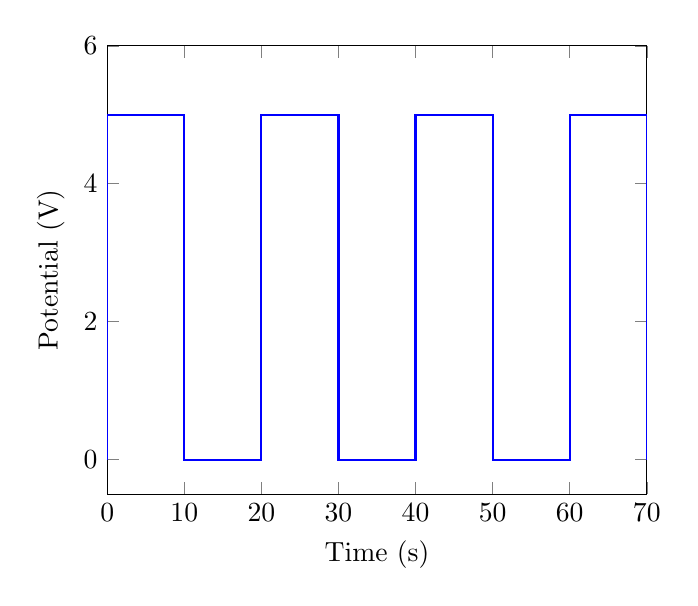
\begin{tikzpicture}
 
    \begin{axis}[
        ylabel={Potential (V)},
        xlabel={Time (s)},
        xmin = 0, xmax = 70,
        ymin = -0.5, ymax = 6]
        \addplot+[thick,mark=none,const plot]
        coordinates
        {(0,0) (0,5) (10,0) (20,5) (30,0) (40,5) (50,0) (60,5) (70,0)};
    \end{axis}
     
  \end{tikzpicture}
  \caption{Idealized plotted square wave}
  \label{fig:figure2}
\end{figure}

Increasing the frequency of the function also changed how long each of the pulses on the oscilloscope.
This setup now let us take a reading on what frequency the human eye can perceive. To do so the
frequency was set to 100Hz (No perceivable flickering), and slowly lowered until flickering could be perceived.

\subsection{Counting}
To enable counting different counting where wired up instead of the LED. They needed a constant Voltage
of 5V so the power supply was used again. All of the different counter circuits offered two pins to connect
a clock. The function generator was connected to those pins as such a timing device. The first circuit had
just two buttons start and reset without any additional pins as well as a bar of LEDs to show the current
count. With it the overall setup was confirmed to be working. 
\newline
\newline
Afterwards the a counting device with a
7-segment display was connected. It offered an additional switch to either use the direct output
of the counting IC or put it through a binary to BCD translation IC. BCD stands for  Binary-Coded-Decimal.
BCD uses 4 bits per decimal digit to represent it. 4 bits are used as $2^4=16 > 9$. 
\newline
\newline
Proceeding we wired up a circuit that counted the number of pulses within a given time period (switchable between
0.1s, 1s or 10s). By connecting the function generator again we could test how many pulses where generated by
it in a given second.
\newline
\newline
Last a counting device with four 7-segment displays was connected, it could count up to 9999 ($10^4$). In
addition it also had a start, stop and a reset button with electrical pins, that if grounded also activated
the corresponding action. The stop button was then wired to a hand-held thumb-actuated button. The function
generator was then set to a 1000Hz such that a value of 1 on the counter would represent 1ms. One person then
covered up the start switch with their hand, reset the counter and prepared to press it. The other person
held the stop button, their job was it to press it as soon as they could see the counter starting to count.
This way the reaction time of the person holding the stop-button could be tested. We both recorded our
reaction-times four times varying the time the person had to wait before the start button was pressed.

\subsection{Measuring Gravity}
With the counting circuits setup and verified we could proceed to use them to measure the gravitational
acceleration on different objects. To do so a drop tower with three gates was used. Additionally two of the
previously introduced four 7-segment counters where used. The gates of the tower where then wired up such
that gate one was connected to the start pin of the counter one, gate 2 to the stop pin of counter one as
well as the start counter of counter two and gate three to the stop pin of counter two. Thus creating a
setup that could count the number of pules passing while a object traveled between the respective gates.
By setting the function generator to produce an output of 1000Hz this could then be translated into time.
With this setup different objects where dropped down the tower. Balls of two sizes and 4 different materials
where used as well as a small pen as an object with minimal air resistance. To get additional precision
the actual produced frequency displayed on the function generator was also recorded to apply it as a
later correction. To improve accuracy further a run with done with the function generator set to 10,000Hz.

\section{Experimental Results}

\subsection{Human perceivable frequencies}

\vspace{0.5cm}
\begin{tabular}{lc}
  Person & Frequency (Hz)\\
  \midrule
  Sidney & 36\\
  Bray & 30\\
\end{tabular}
\vspace{0.5cm}

\subsection{Digital Counting}
\paragraph{BIN/BCD circuit}
While testing the BIN/BCD switchable counting circuit it was observed that the 7-segment display did not
go through the numbers correctly all of the time. If the switch was set to BCD the counting worked correctly
with the display going form 0 to 9 and then resetting. Setting the switch to BIN this did not work properly.
The display was instead counting up to 6 and then did show different numbers in a random seaming way.
\paragraph{Function Generator output verification}
When connecting the function generator to the 1s resetting counter, we set different frequencies on
the function generator and observed what the counter counter showed. The observation where as follows:

\begin{enumerate}
  \item When changing the frequency on the oscilloscope it took a while for the number of counts to
  stabilize.
  \item When pressing any of the buttons or moving the cables of the counting circuit the same happened
  \item Once settled the counter showed the same value as the reading on the oscilloscope up to 1 count
  of difference
\end{enumerate}

\subsection{Reaction Time}

\vspace{0.5cm}
\begin{tabular}{lccccc}
  Person & 1 & 2 & 3 & 4 & 5\\
  \midrule
  Sidney & 242,3 & 225,5 & 156,5 & 163 & 228,7\\
  Bray & 189,5 & 330,5 & 252,9 & 150,2 & 171,1\\
\end{tabular}
\vspace{0.5cm}

\subsection{Gravity}

\begin{tabular}{lcccccc}
  Material & $t_0$ & $t_1$ & Correction & $t_{0_{corrected}}$ & $t_{1_{corrected}}$ & g\\
  \midrule
  Rubber & 0,175 & 0,1 & 0,996015936 & 0,174302789 & 0,099601594 & 9,425604156\\
  Wood & 0,179 & 0,1 & 0,996015936 & 0,178286853 & 0,099601594 & 9,567281072\\
  Plastic & 0,182 & 0,104 & 0,996015936 & 0,1812749 & 0,103585657 & 8,714500884\\
  Wood small & 0,18 & 0,1 & 0,996015936 & 0,179282869 & 0,099601594 & 9,600152381\\
  Glass small & 0,181 & 0,099 & 0,996015936 & 0,180278884 & 0,098605578 & 9,884637057\\
  Metal & 0,181 & 0,099 & 0,996015936 & 0,180278884 & 0,098605578 & 9,884637057\\
  Glass  & 0,18 & 0,099 & 0,996015936 & 0,179282869 & 0,098605578 & 9,853528837\\
  Dart & 0,1441 & 0,097 & 1,005025126 & 0,144824121 & 0,097487437 & 8,302050935\\
  Metal (10kHz)& 0,1765 & 0,0981 & 1,005025126 & 0,177386935 & 0,098592965 & 9,794882365\\

\end{tabular}
\vspace{0.5cm}




\section{Discussion and Analysis}

\subsection{Digital Counting}
The counting circuit s


\subsection{Human perceivable frequencies}


\section{Conclusion}


\end{document}